\chapter{Introduction}

This report shall show the steps taken to simulate the growth of cancer cells in a tissue using the Gompertz Equation to model growth.

Growth for individual cells can be modelled using a differential equation so that the number of cells is a function of time, shown in Equation \ref{eq:1}.
The Gompertz Model of Cell Growth works well in this application because it can accurately model the non-exponential nature of cell growth \autocite{tatroMathematicsCancerFitting2018}.
Once an area has reached its capacity no more tumor cells can form, hence the cells must begin to move through a tissue.
This movement can be simulated using simple random walk algorithms within a grid \autocite{codlingRandomWalkModels2008} as shown in Figure \ref{fig:grid-movement}.

\begin{equation}
    \frac{dN}{dt} = kNln\left(\frac{M}{N} \right) \label{eq:1}
\end{equation}

This paper specifically shall analyze the computational complexity of such models and evaluate the differences between simulation techniques.
The underlying implementation shall be investigated, including random algorithms and accuracy of simulations on computer systems.

Simulations shall use Rust as the programming language, for its performance properties \autocite{adamRustConciseOverview2023}.
It allows for fine control over types, which can be useful for numerical simulations.
Fine-grained benchmarks shall be used to evaluate the performance of the simulations using the criterion library \autocite{heislerBheislerCriterionRs2024}.
Analysis of data generated shall be done using Python with Matplotlib and Numpy.



\begin{figure}[!ht]
    \centering
    \begin{subfigure}{0.4\textwidth}
        \centering
    	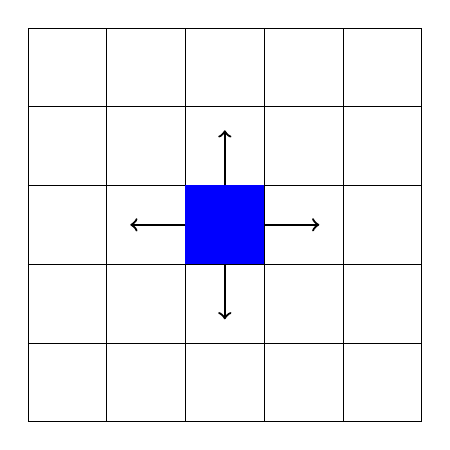
\begin{tikzpicture}
            \draw[step=1cm,black,very thin] (0,0) grid (5,5);
            \fill[blue] (2,2) rectangle (3,3);
        
            % arrows up, down, left, right
            \draw[->, thick] (2.5,3) -- (2.5,3.7);
            \draw[->, thick] (2.5,2) -- (2.5,1.3);
            \draw[->, thick] (2,2.5) -- (1.3,2.5);
            \draw[->, thick] (3,2.5) -- (3.7,2.5);
        \end{tikzpicture}
    	\caption[Square]{Square}
    	\label{fig:grid-movement-square}
    \end{subfigure}
    \begin{subfigure}{0.4\textwidth}
        \centering
    	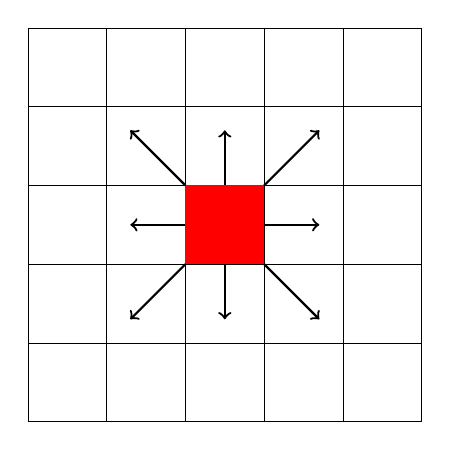
\begin{tikzpicture}
            \draw[step=1cm,black,very thin] (0,0) grid (5,5);
            \fill[red] (2,2) rectangle (3,3);
        
            % arrows up, down, left, right
            \draw[->, thick] (2.5,3) -- (2.5,3.7);
            \draw[->, thick] (2.5,2) -- (2.5,1.3);
            \draw[->, thick] (2,2.5) -- (1.3,2.5);
            \draw[->, thick] (3,2.5) -- (3.7,2.5);

            % arrows diagonals
            \draw[->, thick] (2,3) -- (1.3,3.7);
            \draw[->, thick] (3,3) -- (3.7,3.7);
            \draw[->, thick] (2,2) -- (1.3,1.3);
            \draw[->, thick] (3,2) -- (3.7,1.3);
        \end{tikzpicture}
    	\caption[Diagonal]{Diagonal}
    	\label{fig:grid-movement-diagonal}
	\end{subfigure}
	\caption[Grid movement directions]{Grid movement directions}
    \label{fig:grid-movement}
\end{figure}